\documentclass[10pt,a4paper,twoside]{report}

\input{../../base/BasePackage.sty}
\input{../../base/OptionsListingC++.sty}

\usepackage{units}
\newcommand{\fig}[1]{Figure.~\ref{#1}}

% Mettre des hyperliens dans le pdf
\hypersetup{pdftitle={Projet Observatoire Pierre Auger},
  pdfsubject={Projet d'informatique - Magistère de Physique Fondamentale},
  pdfauthor={Xavier Garrido, LAL,
    <garrido@lal.in2p3.fr>},
  pdfkeywords={rayons cosmiques, observatoire, Pierre Auger}
}

\begin{document}
\renewcommand{\chaptername}{Projet}

\setcounter{chapter}{2}
\chapter{Détection des rayons cosmiques d'ultra-haute énergie :
  Simulation du détecteur de surface}
\label{projet::opa1}

Les rayons cosmiques forment un fond astrophysique de particules
non-thermiques, supposées chargées, dont les énergies observées
s'étendent du MeV jusqu'à quelques \unit[10$^\text{20}$]{eV}. La détection
dès 1962 d'un rayon cosmique d'énergie supérieure à
\unit[10$^\text{20}$]{eV} par John Linsley et ses collaborateurs sur le
site de Volcano Ranch~\cite{linsley}, a soulevé de
multiples questions qui défient encore la physique contemporaine. Si
l'existence de rayons cosmiques à de telles énergies a été confirmée
par d'autres expériences, ni les nombreux travaux théoriques, ni les
quelques données expérimentales disponibles à ce jour, ne permettent
de comprendre complètement l'origine et la nature de ce rayonnement
hautement énergétique.

La problématique du rayonnement cosmique, en particulier de sa
composante à ultra-haute énergie ($E\geq\unit[10^{18}]{eV}$), se
présente à la fois sous des aspects théoriques,
phé\-no\-mé\-no\-lo\-gi\-ques et observationnels. D'une part, les
astrophysiciens peinent à identifier les sources et les mécanismes
d'accélération capables de porter des protons ou des noyaux du milieu
interstellaire à des énergies aussi extrêmes. D'autre part,
l'interaction de ces astroparticules avec le fond diffus cosmologique,
qui intervient lors de leur propagation dans l'Univers, devrait
entraîner la suppression de leur flux au delà de
$\unit[10^{20}]{eV}$. Cette caractéristique du spectre en énergie
connue sous le nom de coupure GZK~\cite{greisen, zatsepin}, est
étroitement liée à toute la physique spéculative qui gravite autour de
l'existence même de ces rayons cosmiques d'ultra-haute
énergie~(RCUHE). Enfin, la rigidité de ces particules, à savoir le
rapport de leur énergie sur leur charge, conjuguée à la supposée
faible intensité du champ magnétique extragalactique et à la
connaissance raisonnable de sa composante galactique, rendent
pertinentes les tentatives de corrélation entre leurs directions
d'arrivées et leurs sites de production.

La principale limitation technique tient à la rareté des RCUHEs
$-$~typiquement 1 particule par km$^2$ et par siècle à
$\unit[10^{20}]{eV}$~$-$ impliquant la mise en \oe uvre d'une surface
de détection exceptionnelle pour recueillir un nombre d'événements
statistiquement représentatif. Par ailleurs, l'observation des rayons
cosmiques se fait au travers de l'étude des cascades de particules
secondaires, conséquence du passage de ces corpuscules extrêmes au
sein de l'atmosphère : les propriétes du rayonnement cosmique sont
donc indirectement déduites de l'étude des gerbes
atmosphériques. Grâce à la combinaison d'un réseau de 1600 cuves à
effet Cherenkov associé à 24 télescopes de fluorescence,
l'Observatoire Pierre Auger peut observer simultanément le
dévelop\-pement longitudinal et latéral des gerbes atmosphériques. Le
couplage de ces deux techniques permet d'affiner les reconstructions
géométriques, d'intercalibrer les détecteurs et d'évaluer, en
conséquence, les éventuels biais inhérents à chaque mode de
détection. En outre, la surface couverte par le détecteur de surface
voisine de $\unit[3000]{km^2}$ fait de cet instrument le plus grand
détecteur de rayons cosmiques jamais construit.

\begin{figure}
  \centering
  \begin{tabular}{cc}
    \includegraphics[scale=0.4]{./plot/AugerEvent_200812301774}&
    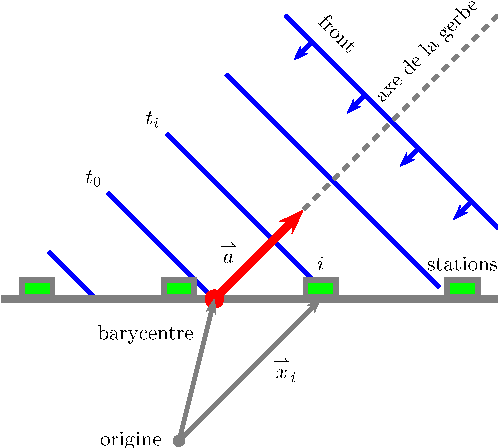
\includegraphics[scale=0.8]{./plot/planeFront}
  \end{tabular}
  \caption{\textbf{\label{fig::rec}Vue 3D d'un événement hybride observé par
      l'Observatoire Pierre Auger~(figure de gauche). Description
      géométrique du développement du front de gerbe~(figure de droite).}}
\end{figure}

\section{Présentation du projet}

Le but de ce projet est de simuler la réponse du \textbf{détecteur de
  surface} puis de reconstruire les propriétés géométriques (position
du point d'impact, énergie) des gerbes atmosphériques. Le détecteur de
surface se présente sous la forme d'un réseau de maille triangulaire
où chaque station est séparée de ses voisines par une distance de
\unit[1.5]{km}. Au passage des particules secondaires de la gerbe
atmosphérique, chaque station mesure le temps d'arrivée et l'amplitude
du signal. Grâce à ces données, on peut ainsi déterminer :

\begin{enumerate}

\item[\textbullet] \textbf{la direction de la gerbe} à partir des
  temps d'arrivées de chacune des cuves ayant déclenchés. Trois temps
  sont ainsi nécessaires pour déterminer le plan de front de
  gerbe~(\emph{cf.}~\fig{fig::rec}),

\item[\textbullet] \textbf{les coordonnées du point d'impact} sont
  calculées , en première approximation, comme le centre de gravité
  des positions des cuves pondérées par leur signal,

\item[\textbullet] \textbf{l'énergie de la particule primaire} est
  mesurée grâce à la distribution latérale de signal : la densité de
  particule et donc le signal généré dans chacune des cuves décroît
  avec la distance à l'axe de la gerbe $r$ selon une loi de
  puissance. La valeur du signal à \unit[1000]{m} dont l'unité est le
  VEM (\emph{Vertical Equivalent Muon}) permet alors de déterminer
  l'énergie du rayon cosmique incident : \unit[8]{VEM} sont ainsi
  équivalents à une gerbe de \unit[10$^\text{18}$]{eV}.

\end{enumerate}

\subsection{Génération et simulation d'événement}

Un événement est caractérisé par l'énergie~$E$ de la particule
primaire, sa direction ($\theta$, $\phi$) ainsi que le point d'impact~$I$
($x_i$, $y_i$). La première partie du projet consiste en la simulation
d'une part, de gerbes atmosphériques et d'autre part, de la réponse du
détecteur de surface. La génération des événements consiste à tirer
aléatoirement des valeurs pour les variables ($E, \theta, \phi, x_I,
y_I$) : les valeurs d'énergie $E$ seront uniformément comprises entre
\unit[10$^\text{18}$]{eV} et \unit[10$^\text{20}$]{eV} tandis que
l'angle $\theta$ sera généré selon une distribution en $\cos\,\theta$.

\begin{figure}
  \centering
  \includegraphics[scale=1.]{./plot/sd}
  \caption{\textbf{\label{fig::sd}Réprésentation d'un réseau de
      surface constitué de 3 cuves.}}
\end{figure}

Dans un premier temps, le détecteur de surface sera uniquement
constitué de 3~cuves qui formeront une maille élémentaire du
réseau~(\emph{cf.}~\fig{fig::sd}). Chaque cuve sera atteinte à un
temps $t_i$ proportionnel à la distance séparant la cuve de l'axe de la
gerbe

\begin{equation*}
  t_i = \frac{IH_i}{c} = \frac{\vec{IS_i}\cdot\vec{a}}{c}
\end{equation*}
où $\vec{a}=(1,\theta, \phi)$
Le signal $s_i$, exprimé en VEM, sera simulé en tenant compte de la
distribution latérale du signal selon

\begin{equation*}
  s_i = \left.8\right|_\text{\tiny VEM}\times\frac{E}{\unit[10^{18}]{eV}}\times\left(\frac{d_\perp^i}{\unit[1000]{m}}\right)^{-1.3}
\end{equation*}
où $d_\perp^i = \sqrt{IS_i^2 - IH_i^2}$ est la distance perpendiculairement à
l'axe de la gerbe.

\subsection{Reconstruction des événements}

\'Etant donné les informations déduites du détecteur de surface, on
déterminera le point d'impact de la gerbe en calculant le barycentre
des positions des cuves pondérées par le signal. L'énergie de la gerbe
sera calculée en ajustant la distribution latérale du signal.

Les résultats obtenus seront comparés aux données simulées en générant
un grand nombre d'événement. On discutera les biais ainsi que la
résolution en énergie en établissant les distributions des écarts
relatifs en énergie et celles du point d'impact.

Dans un second temps, on pourra considérer un réseau de cuve plus
dense et on évaluera l'évolution des précédentes quantités en
fonction du nombre de stations.

\def\etal{\textit{et al.}}

\renewcommand{\bibname}{References}

\begin{thebibliography}{9}
  \bibliographystyle{unsrt}

\bibitem{linsley} J.~Linsley, {\em Evidence for a Primary Cosmic-Ray
  Particle with Energy 10$^{20}$ eV}", Physical Review Letters,
  vol. 10, pp 146-148 (1963)

\bibitem{greisen} K.~Greisen, {\em End to the Cosmic-Ray Spectrum ?},
  Physical Review Letters, vol. 16, pp 748-750 (1966)

\bibitem{zatsepin} G.~T.~Zatsepin and V.~A.~Kuz'min, {\em Upper Limit
  of the Spectrum of Cosmic Rays}, Soviet Journal of Experimental and
  Theoretical Physics Letters, vol. 4, pp 78 (1966)

\end{thebibliography}


\end{document}

% Local Variables:
% mode: latex
% coding: utf-8-unix
% End:
